\documentclass[12pt,a4paper]{article}
\usepackage[utf8]{inputenc}
\usepackage[russian]{babel}
\usepackage[OT1]{fontenc}
\usepackage{amsmath}
\usepackage{amsfonts}
\usepackage{amssymb}
\usepackage{graphicx}
\usepackage{wrapfig}
\usepackage{subfigure}
\usepackage[left=2cm,right=2cm,top=2cm,bottom=2cm]{geometry}
\author{Григорий Чирков}
\title{Лабораторная работа № 2.1 \\
		 Опыт Франка-Герца}
\begin{document}
\maketitle

\section{Теория}
Опыт Франка-Герца -- это один из простейших экспериментов, доказывающих существование дискретных уровней энергии атомов.

\begin{wrapfigure}{r}{0.5\linewidth} \label{scheme} 
\vspace{-5ex}  
 \center{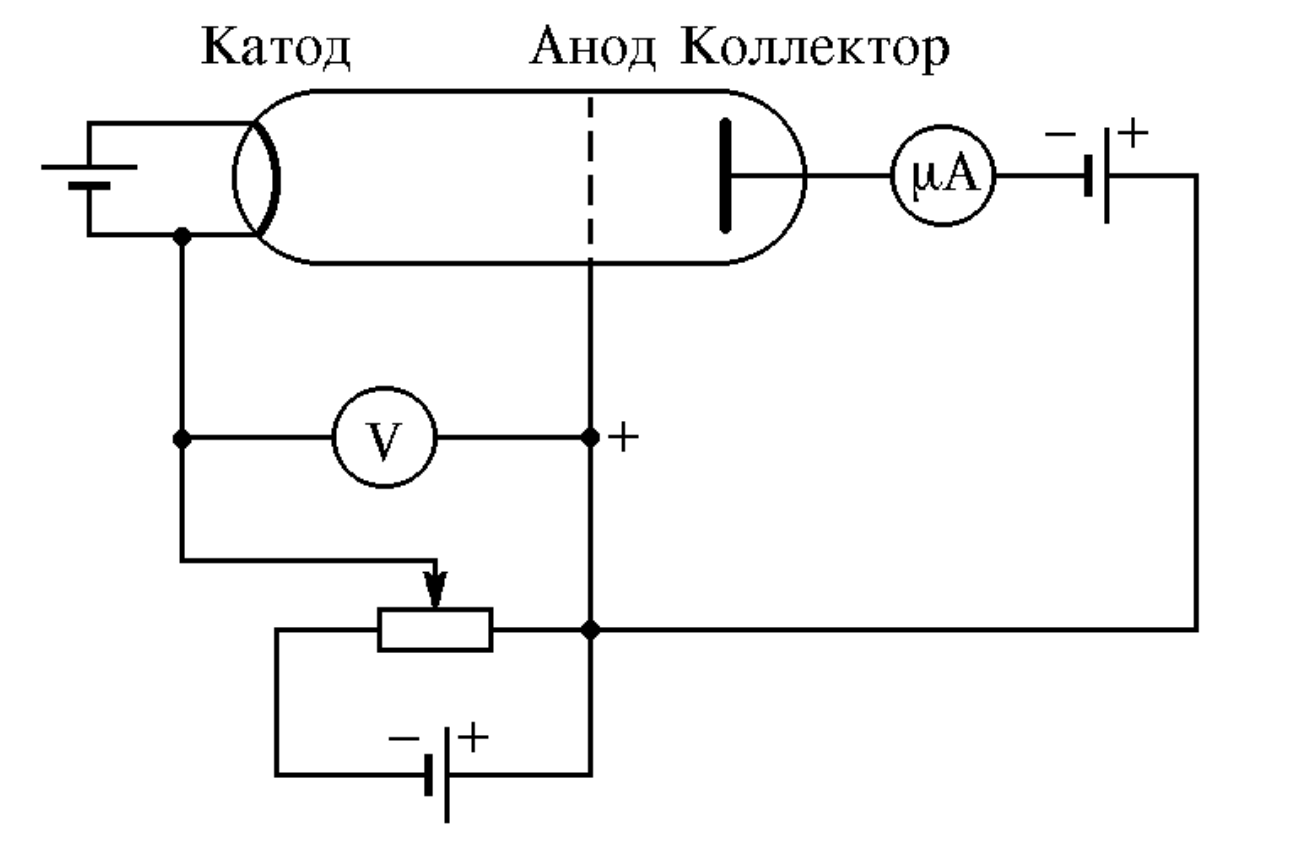
\includegraphics[width=.7\linewidth]{1.png}}
\caption{Принципиальная схема опыта}
\end{wrapfigure}

Разреженный одноатомный газ заполняет трехэлектродную лампу(рис. \ref{scheme}).  Электроны, испускаемые разогретым катодом, ускоряютсяв постоянном электрическом поле, созданным между катодом и сетчатым анодом лампы. ередвигаясь от катода к аноду, электроны сталкиваются с атомами гелия. Если энергия электрона, налетающего на атом, недостаточна для того, чтобы перевести его в возбужденное состояние, то возможны только упругие столкновения, при которых электроны почти не теряют энергии, так как их масса в тысячи раз меньше массы атомов. 


По мере увеличения разности потенциалов между анодом и катодом энергия электронов увеличивается и, в конце концов, оказывается достаточной для возбуждения атомов. При таких -- неупругих -- столкновениях кинетическая энергия налетающего электрона передается одному из атомных электронов, вызывая его переход на свободный энергетический уровень (возбуждение) или совсем отрывая его от атома (ионизация).

Третьим электродом лампы является коллектор. Между ним и анодом поддерживается небольшое задерживающее напряжение (потенциал коллектора меньше потенциала анода). Ток коллектора, пропорциональный числу попадающих на него за секунду электронов, измеряется микроамперметром.

\begin{wrapfigure}{l}{0.5\linewidth} \label{dependency} 
\vspace{-6ex}  
 \center{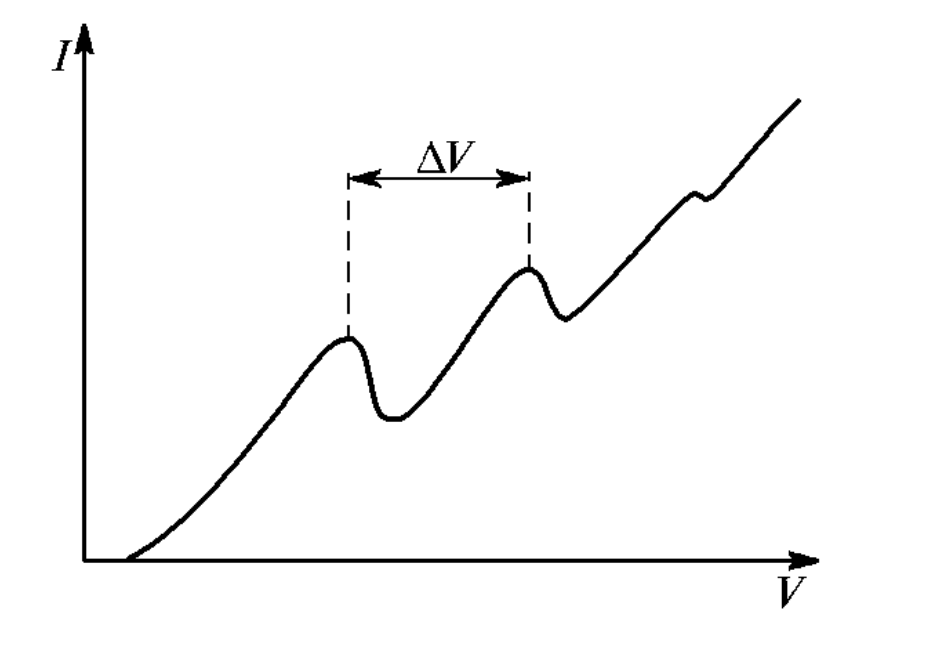
\includegraphics[width=.7\linewidth]{2.png}}
\caption{Зависимость тока коллектора от напряжения на аноде}
\end{wrapfigure}

При увеличении потенциала анода ток в лампе вначале растет, подобно тому как это происходит в вакуумном диоде(рис. \ref{dependency}). Однако, когда энергия электронов становится достаточной для возбуждения атомов, ток коллектора резко уменьшается. Это происходит потому, что при неупругих соударениях с атомами электроны почти полностью теряют свою энергию и не могут преодолеть задерживающего потенциала между анодом и коллектором. При дальнейшем увеличении потенциала анода ток коллектора вновь возрастает: электроны, испытавшие неупругие соударения, при дальнейшем движении к аноду успевают набрать энергию, достаточную для преодоления задерживающего потенциала. Следующее замедление роста тока происходит в момент, когда часть электронов неупрого сталкивается с атомами два раза: первый раз посередине пути, второй -- у анода и т.д. Таким образом, на кривой зависимости тока коллектора от напряжения анода имеется ряд максимумов и минимумов, отстоящих друг от друга на равные расстояния $\Delta V$.

\section{Экспериментальная установка}

\begin{wrapfigure}{r}{0.5\linewidth} \label{fullscheme} 
\vspace{-5ex}  
 \center{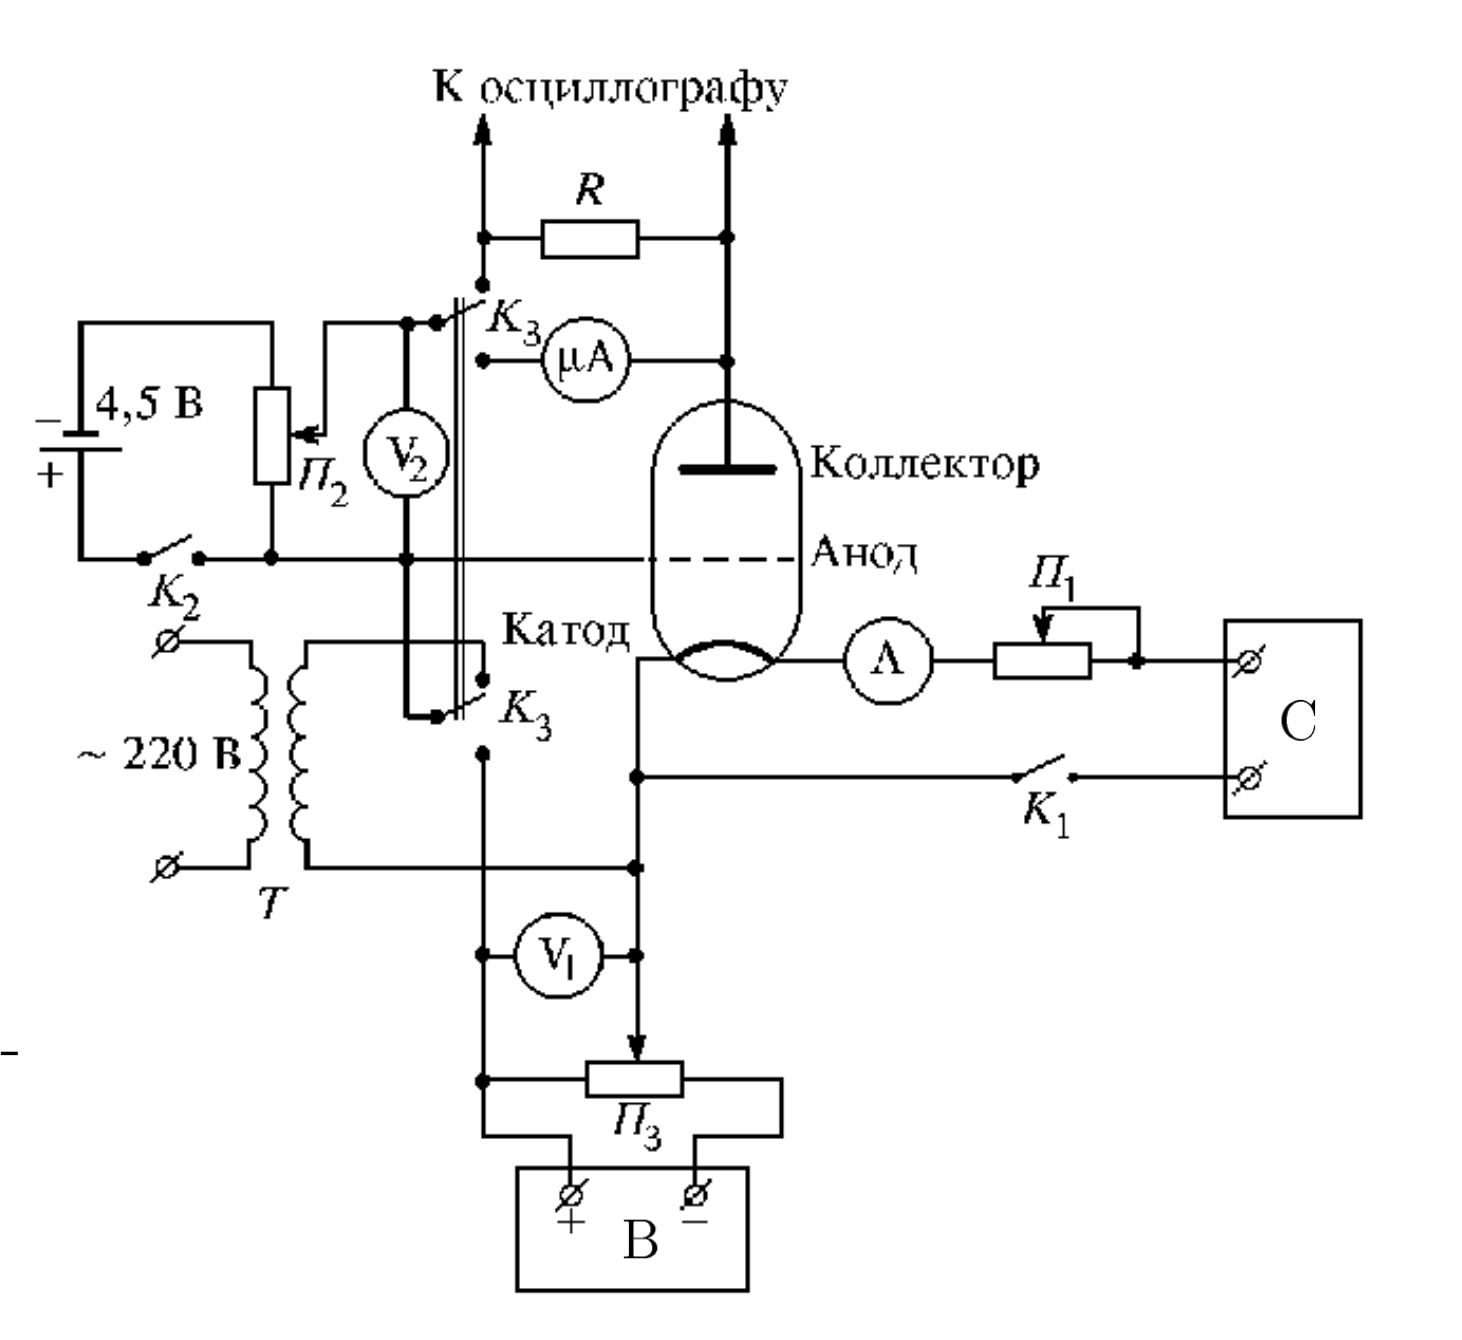
\includegraphics[width=.7\linewidth]{3.png}}
\caption{Схема установки}
\end{wrapfigure}


Для опыта используется лампа ионизационного манометра ЛМ-2, заполненная гелием до давления $\sim 1$ Торр. Напряжение накала подается от источника питания C. Ток накала контролируется амперметром А. Ускоряющее напряжение подается на анод от выпрямителя B. Ток в цепи коллектора регистрируется микроамперметром.

Схему можно переключать из статического режима измерений в динамический. При нем ускоряющий потенциал подается с понижающего трансформатора Т( 220/50 В), а ток коллектора регистрируется осциллографиом, подключенным к нагрузочному резистору R. 

\section{Ход работы}

\begin{enumerate}
\item В динамическом режиме работы установки получить фигуры Лиссажу на осциллографе, подавая на ось Х -- напряжение с анода, а на ось У -- ток коллектора. Измерить расстояние между максимумами $\Delta V$. Повторить измерения для значений задерживающего напряжения 4, 6, 8 В.
\item В статическом режиме работы установки снять зависимость тока коллектора от напряжения на аноде для тех же значений задерживающего напряжения.
\end{enumerate}

\newpage

\section{Обработка полученных результатов}

\begin{enumerate}
\item Динамический режим:

\begin{figure}[h]  
\vspace{4ex} 
\centering 
\subfigure[]
{
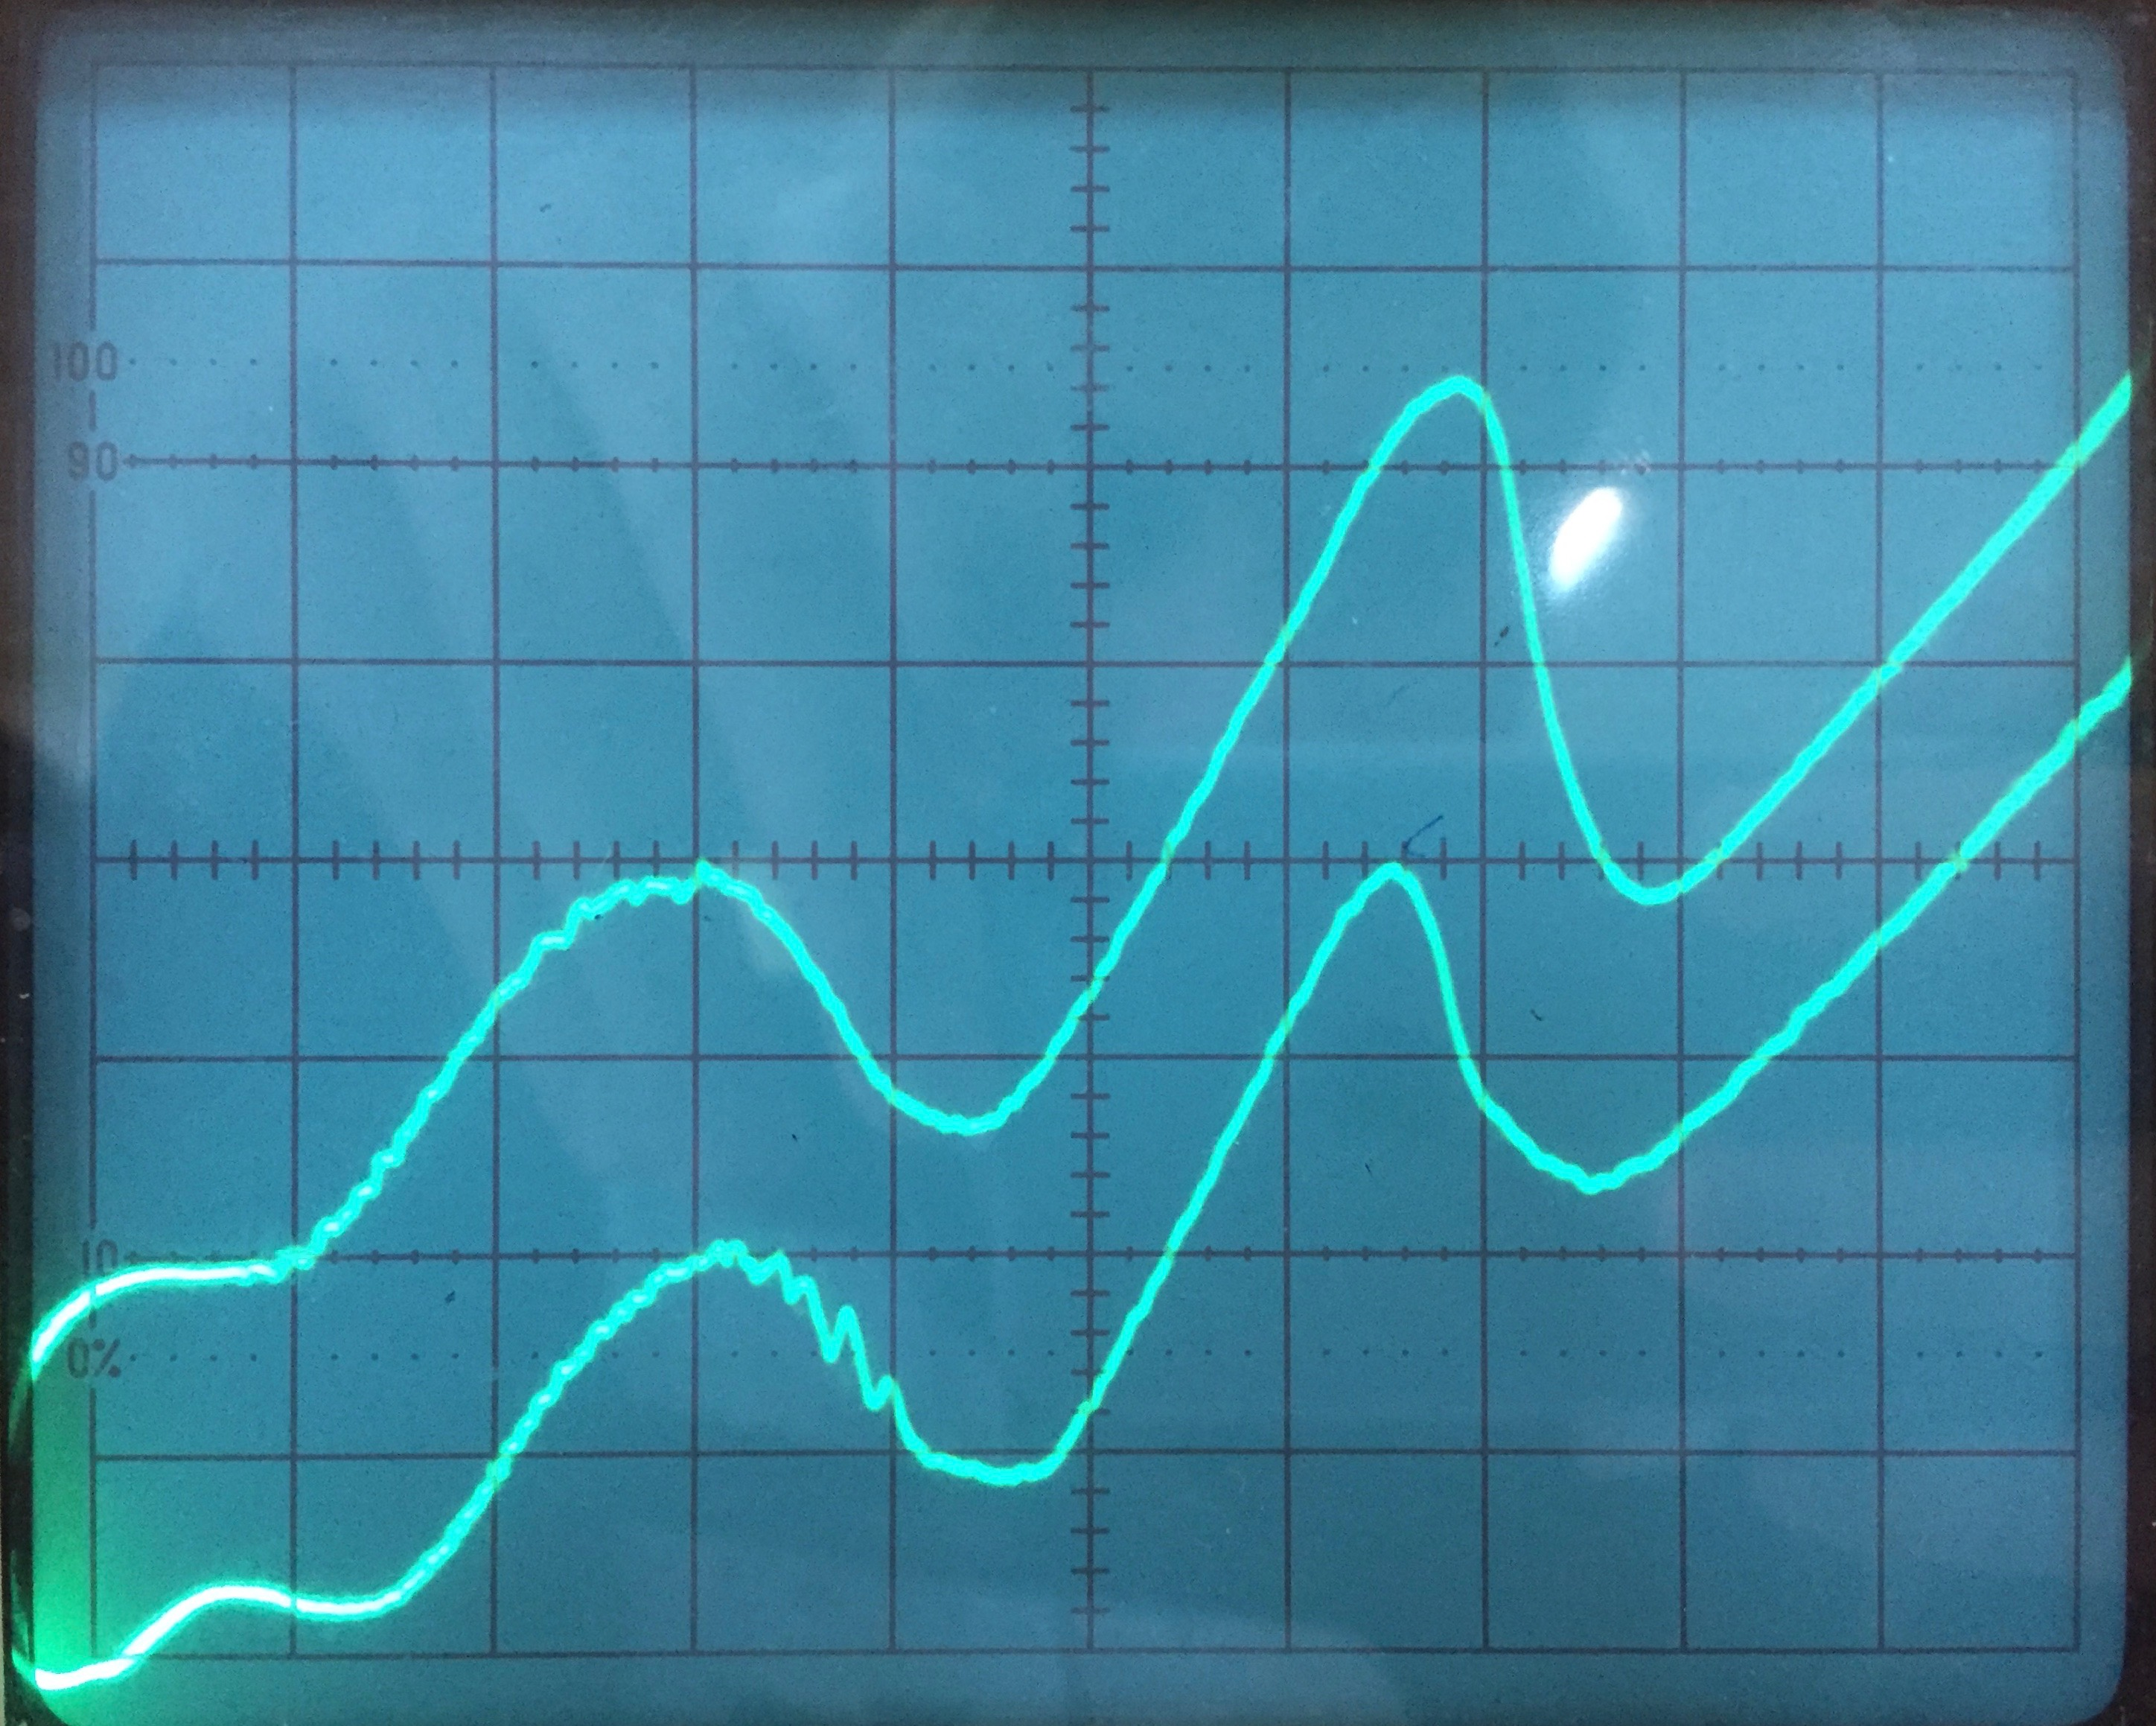
\includegraphics[width=0.25\linewidth]{4V.jpg} \label{fig:actuatorscouplingSheme_decoupledcase} 
}  
\hspace{4ex}
\subfigure[]
{
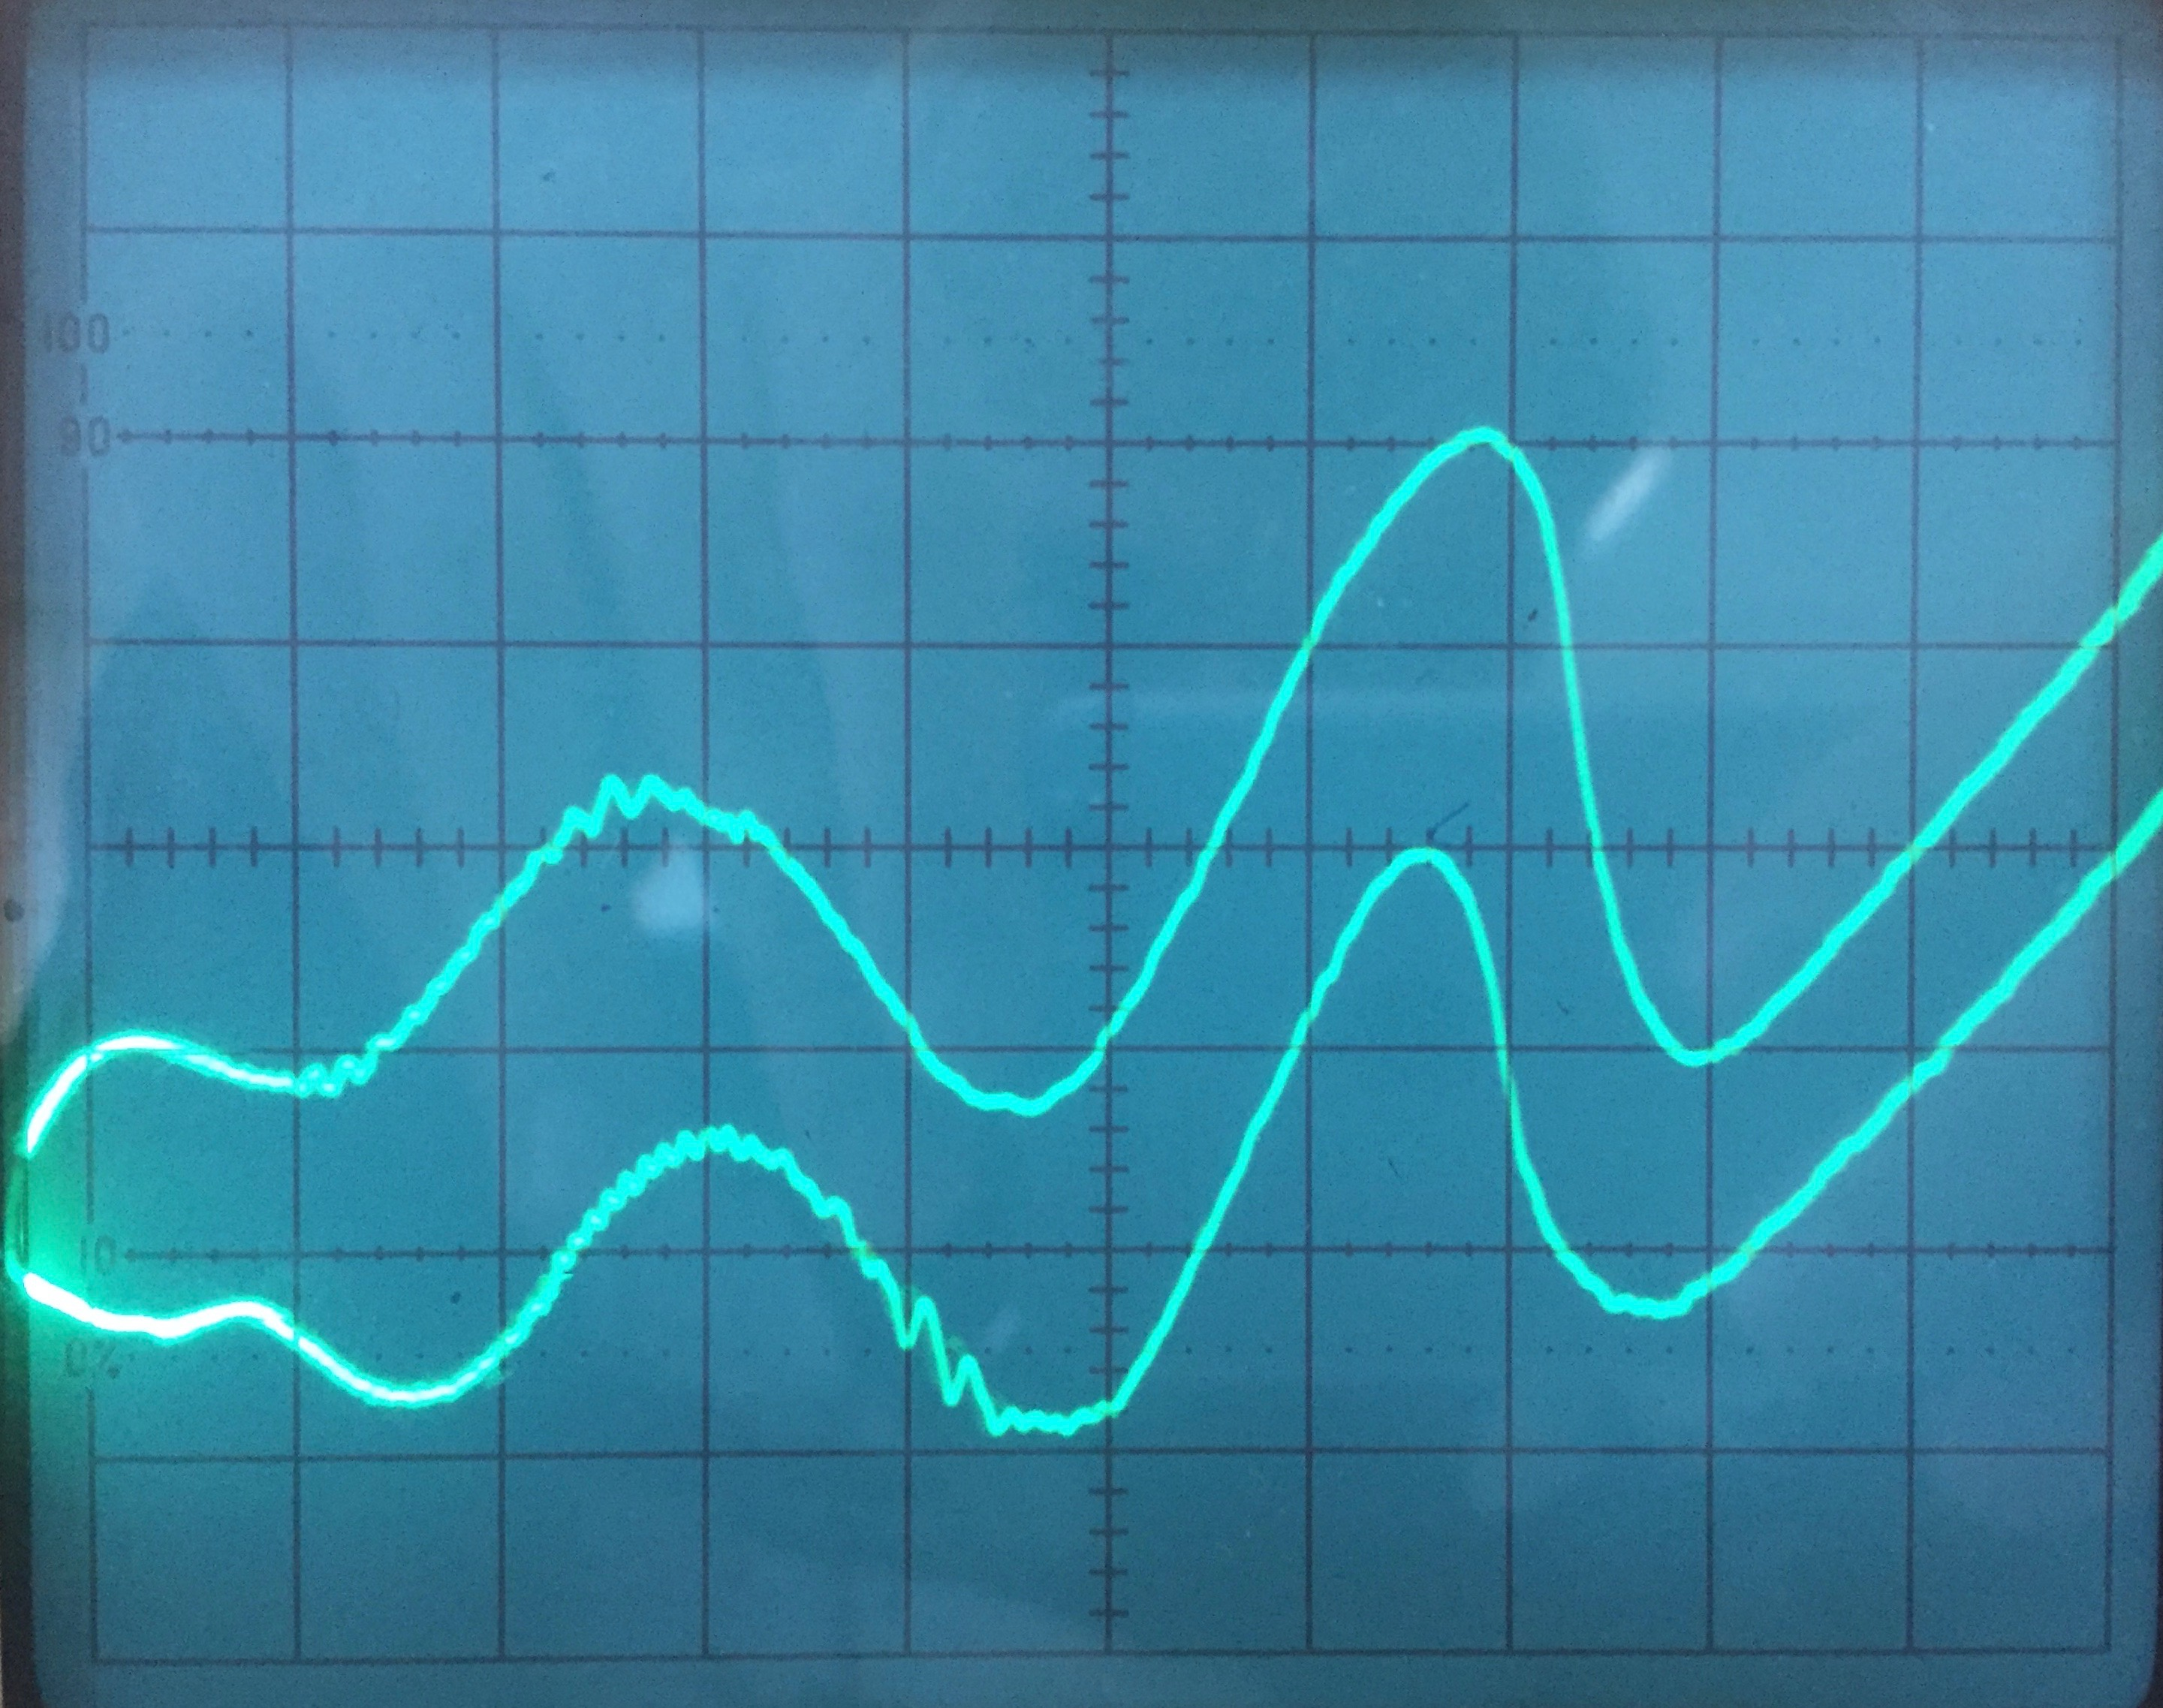
\includegraphics[width=0.25\linewidth]{6V.jpg} \label{fig:actuatorscouplingSheme_nearestcoupledcase} 
}
\hspace{4ex}
\subfigure[]
{ 
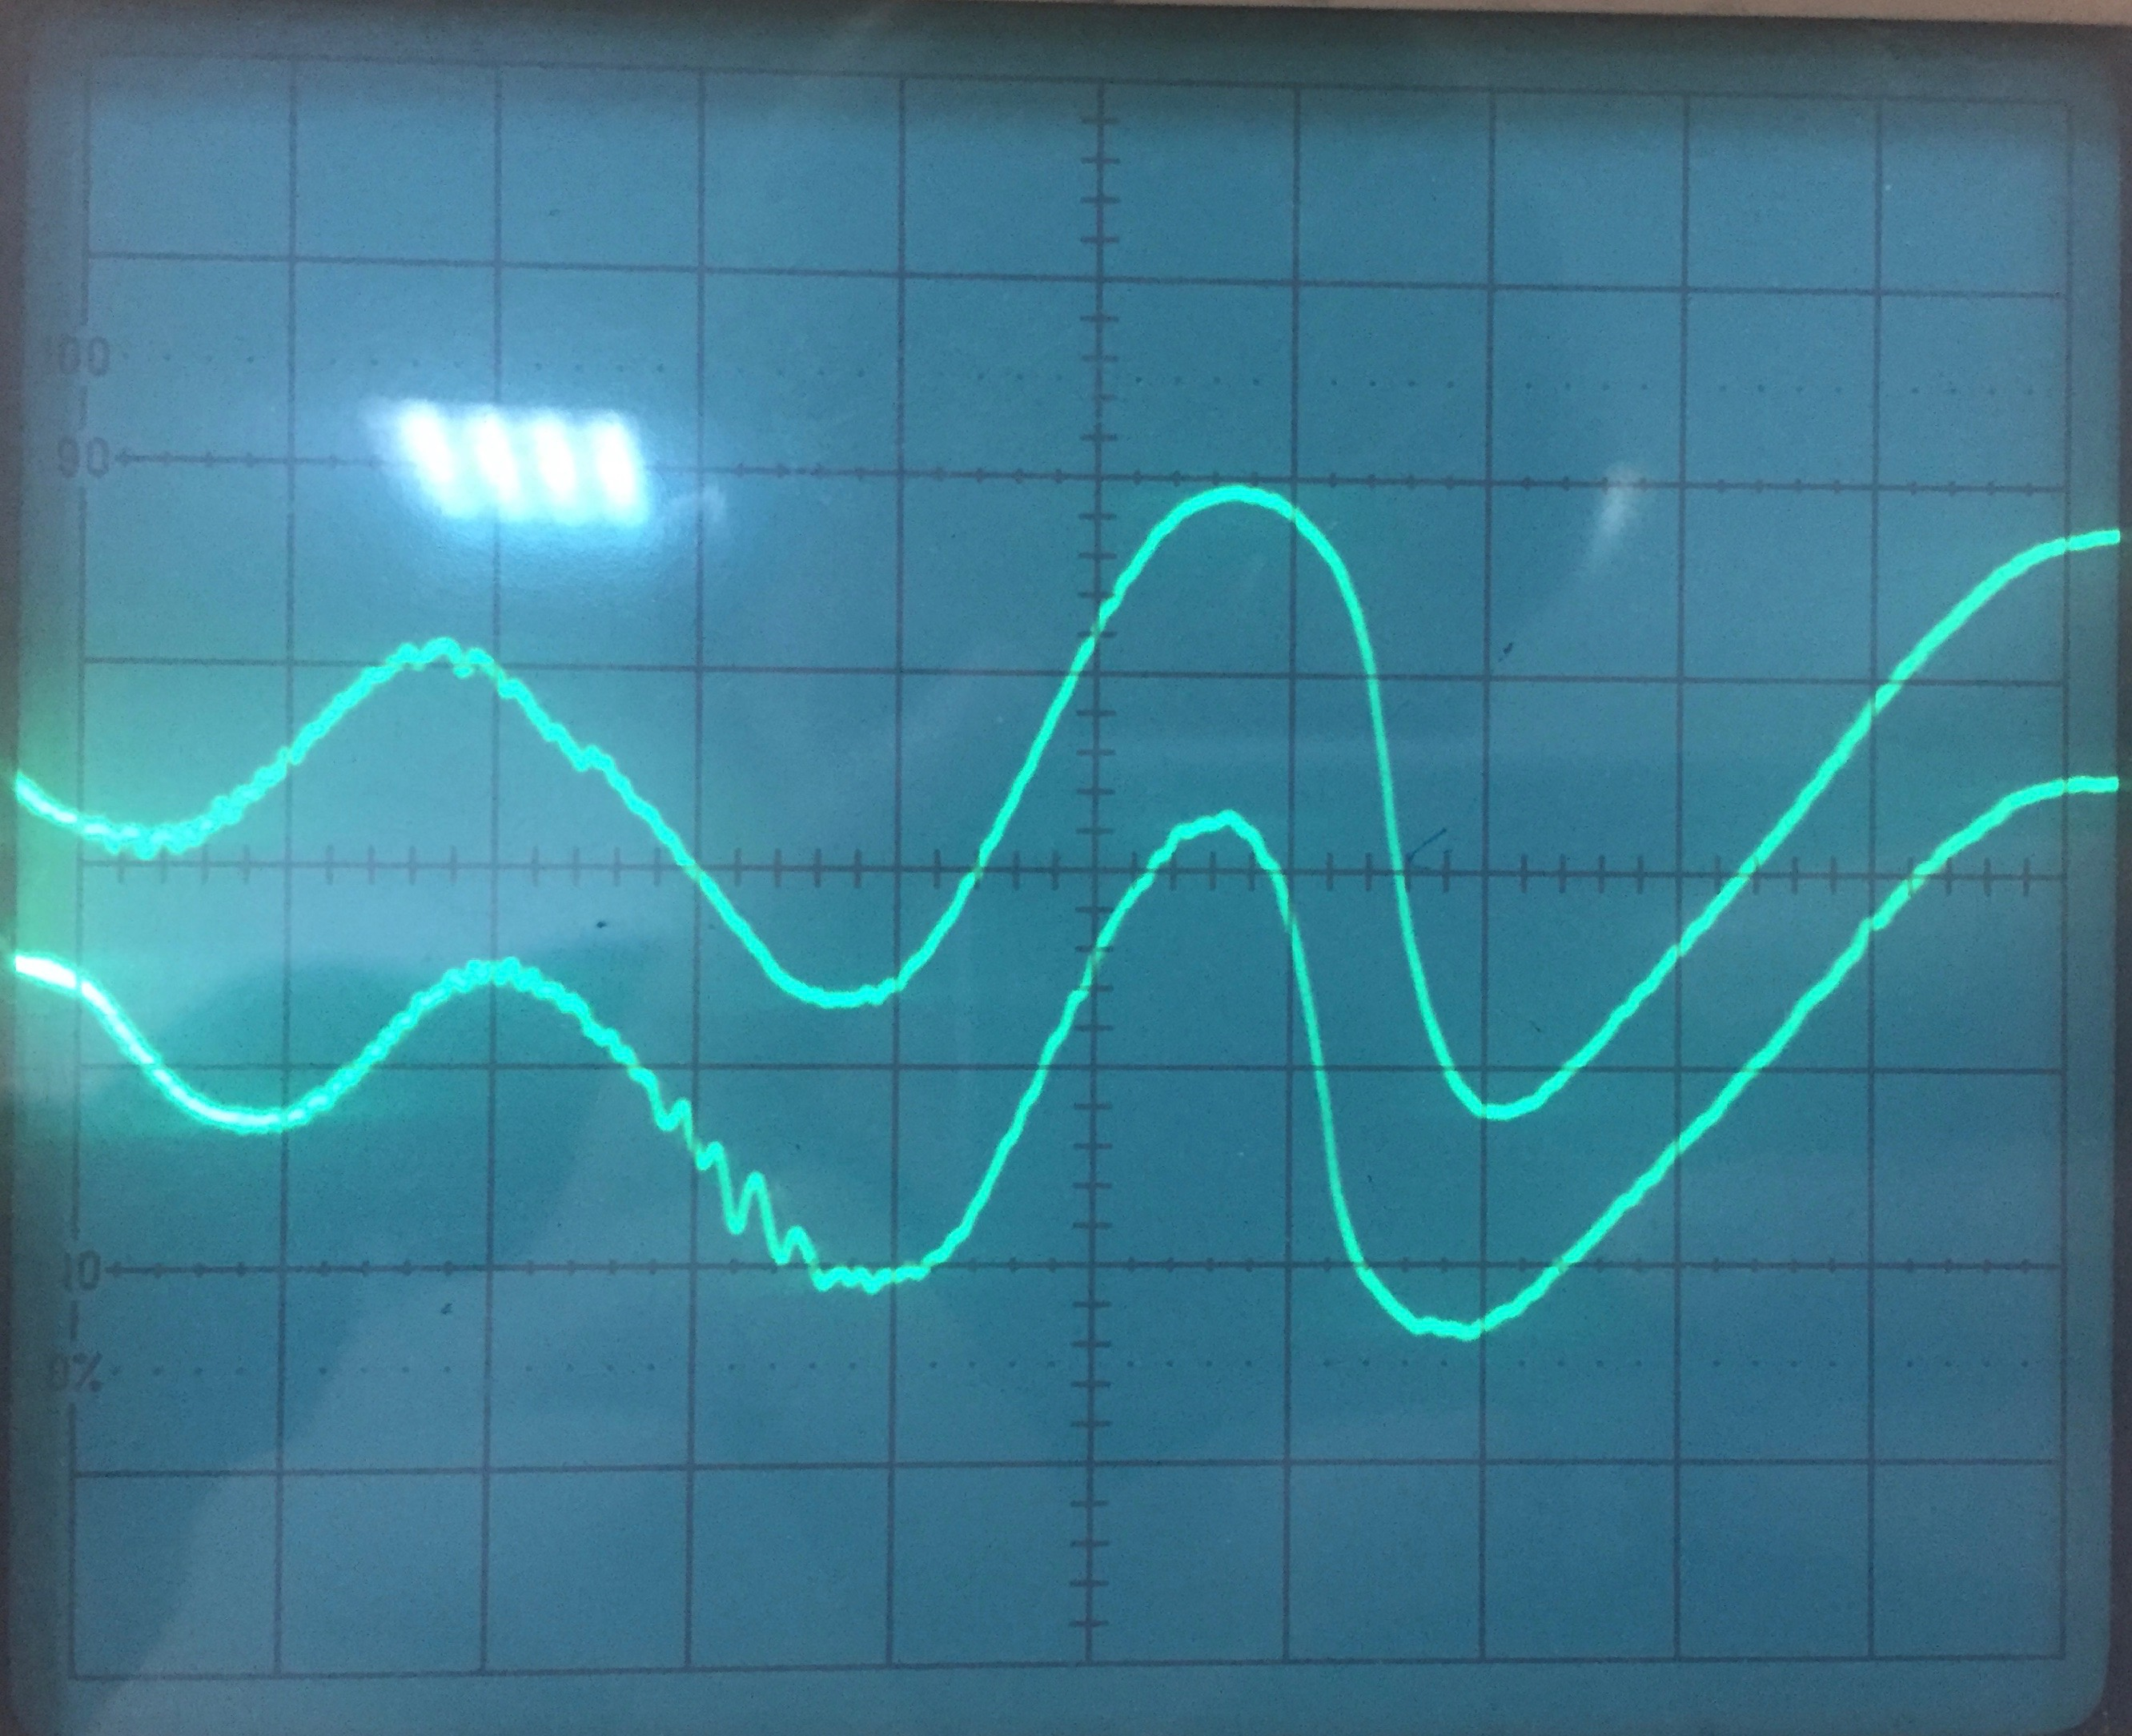
\includegraphics[width=0.24\linewidth]{8V.jpg} \label{fig:actuatorscouplingSheme_nearestcoupled_and_diag_case} }  
\caption{Зависимость тока коллектора от напряжения на аноде в динамическом режиме при запирающем напряжении: \subref{fig:actuatorscouplingSheme_decoupledcase} 4В; \subref{fig:actuatorscouplingSheme_nearestcoupledcase}  6В; \subref{fig:actuatorscouplingSheme_nearestcoupled_and_diag_case}   8В.} \label{fig:threeDMcases}
\end{figure}


\begin{itemize}

\begin{minipage}{0.3\textwidth}
	\item 4В:
	\begin{eqnarray*}
		\Delta V_{max} = 19V \\
		\Delta V_{min} = 18V
	\end{eqnarray*}
\end{minipage}
\begin{minipage}{0.3\textwidth}
  	\item 6В:
	\begin{eqnarray*}
		\Delta V_{max} = 20V \\
		\Delta V_{min} = 17V
	\end{eqnarray*}
\end{minipage}
\begin{minipage}{0.3\textwidth}
	\item 8В:
	\begin{eqnarray*}
		\Delta V_{max} = 20V \\
		\Delta V_{min} = 18V
	\end{eqnarray*}
\end{minipage}

\end{itemize}

Получаем:
\begin{eqnarray*}
E_1 = e <\Delta V_{max}> = 19.7 eV \\
\sigma_{\Delta V} = 0.57 eV
\end{eqnarray*}

\item Статический режим:
\begin{figure}[h!]
 \center{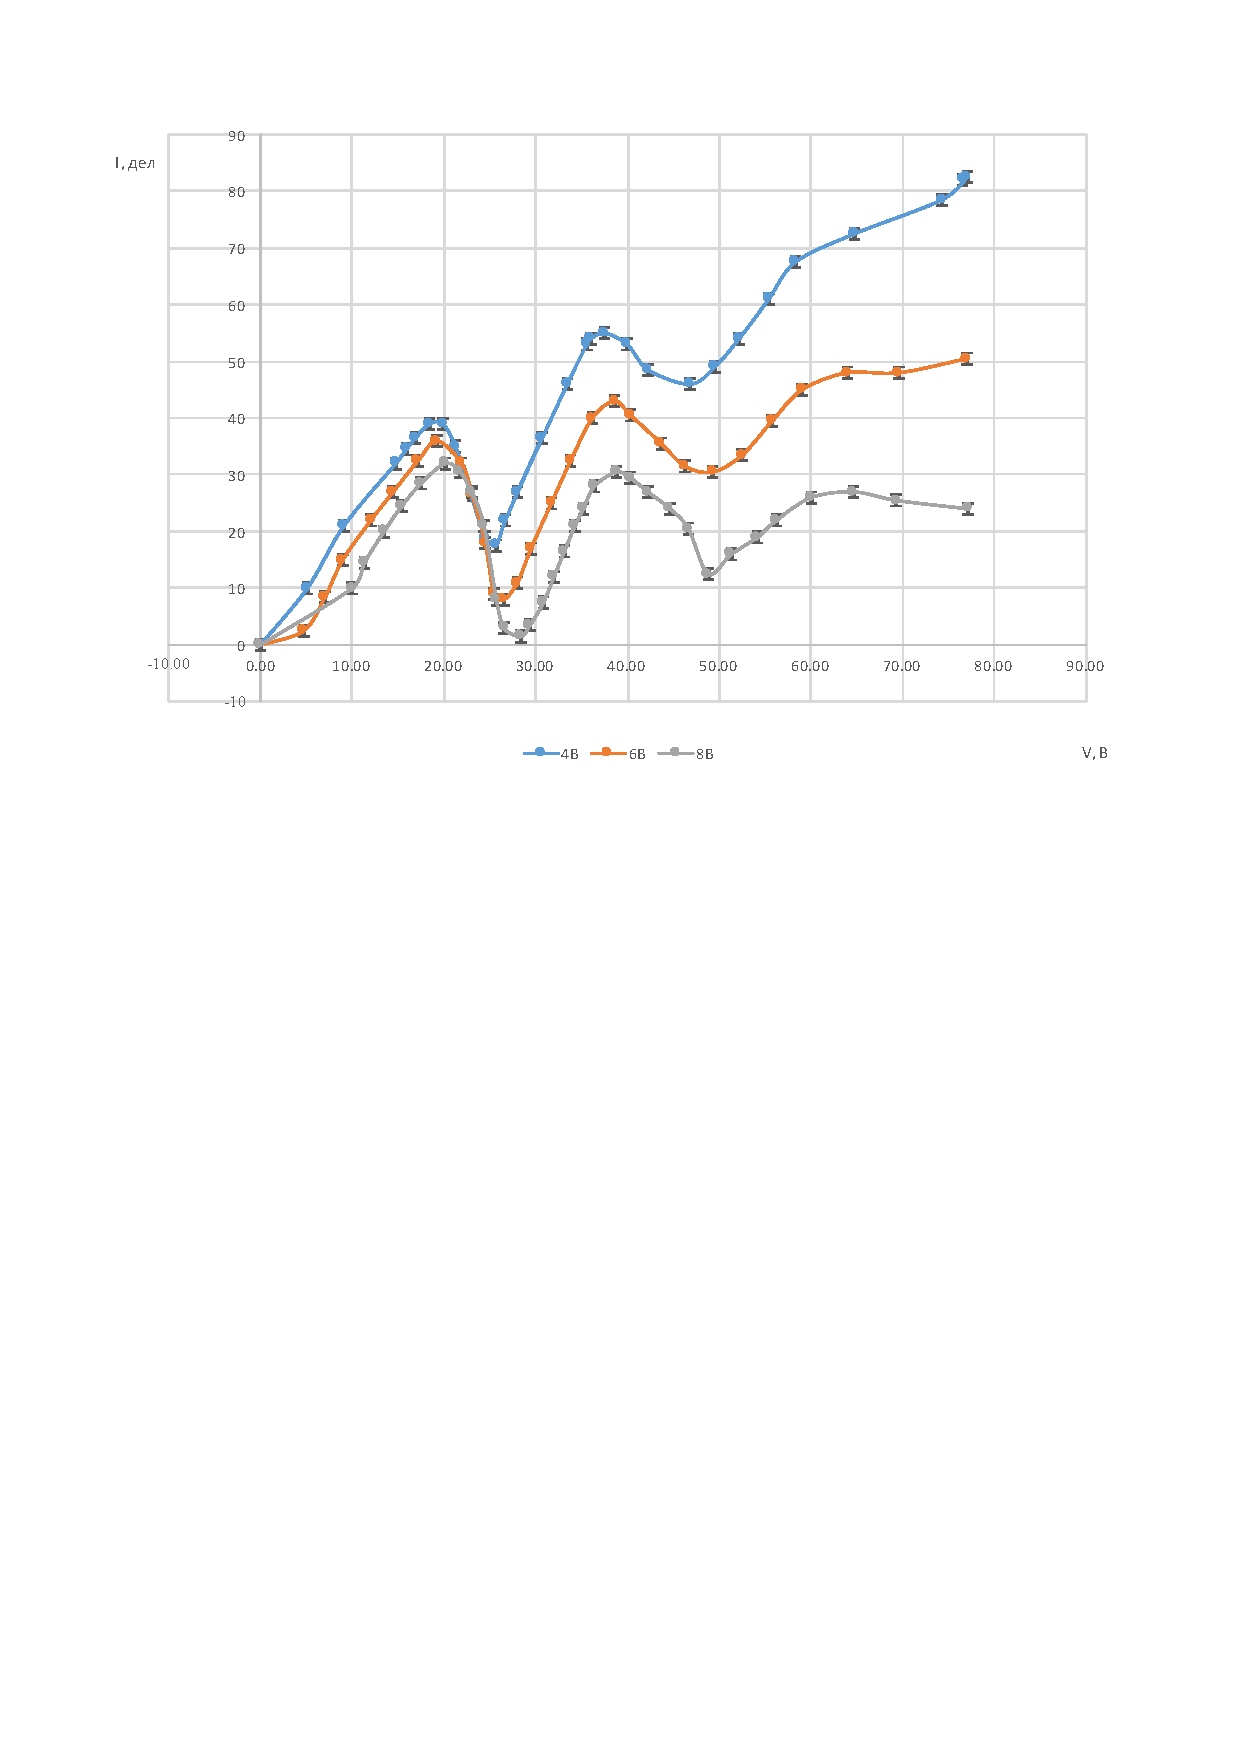
\includegraphics[width=\linewidth]{graph.pdf}}
\caption{Семейство зависимостей тока коллектора от напряжения на аноде}
\end{figure}

По данным графиков:

\begin{itemize}

\begin{minipage}{0.3\textwidth}
	\item 4В:
	\begin{eqnarray*}
		\Delta V_{max} = 19.21V \\
		\Delta V_{min} = 21.12V
	\end{eqnarray*}
\end{minipage}
\begin{minipage}{0.3\textwidth}
  	\item 6В:
	\begin{eqnarray*}
		\Delta V_{max} = 19.40V \\
		\Delta V_{min} = 22.74V
	\end{eqnarray*}
\end{minipage}
\begin{minipage}{0.3\textwidth}
	\item 8В:
	\begin{eqnarray*}
		\Delta V_{max} = 19.91V \\
		\Delta V_{min} = 20.40V
	\end{eqnarray*}
\end{minipage}

\end{itemize}

Получаем:
\begin{eqnarray*}
E_1 = e <\Delta V_{max}> = 19.51 eV \\
\sigma_{\Delta V} = 0.36 eV
\end{eqnarray*}

\end{enumerate}

\newpage
\section{Вывод}
В ходе опыта была прослежена дискретная природа энергитических уровней атома гелия. Были получены значения первого энергетического уровня атома гелия в динамическом ($19.70 \pm 0.57 eV$) и статическом ($19.51 \pm 0.36 eV$) режимах. Полученные результаты совпадают с табличным значением ($19.82 eV$) с точностью до погрешности.
\end{document}